\documentclass{ecnreport}

\stud{Option Robotique, EMARO-ARIA M1}
\topic{Computer Vision}

\begin{document}

\inserttitle{Computer Vision Lab}

\insertsubtitle{Labs 3-4: Calibration and pose computation}



\section{Content of this lab}

The goal is this lab is to perform camera calibration and pose computation. Do to so, we will use two C++ libraries:
\begin{itemize}
 \item OpenCV\footnote{Open source Computer Vision, http://opencv.org} to read images from files or camera, and perform low-level image processing
 \item ViSP\footnote{Visual Servoing Platform, http://visp.inria.fr} to manipulate 3D points, camera pose and use vectors and matrices.
\end{itemize}
The actual classes that are used are detailed in Appendix \ref{sec:classes}.

\subsection{The cameras}

Several IEEE-1394 Firewire cameras are available for this lab. Some of them have a low distortion while others are fish-eye cameras. We will consider the 
same framework to calibrate and perform pose computation for both, that is virtual visual servoing (VVS).

\subsection{Calibration landmarks}

Camera calibration and pose computation usually require to observe known objects. In our case we will consider a grid composed of 6$\times$6 points and
the OpenCV chessboard (see \Fig{fig:landmarks}).

\begin{figure}[h!]
 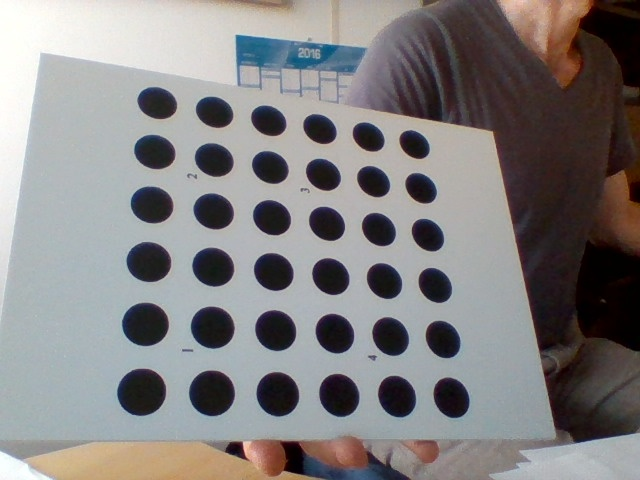
\includegraphics[width=.45\linewidth]{grid} ~~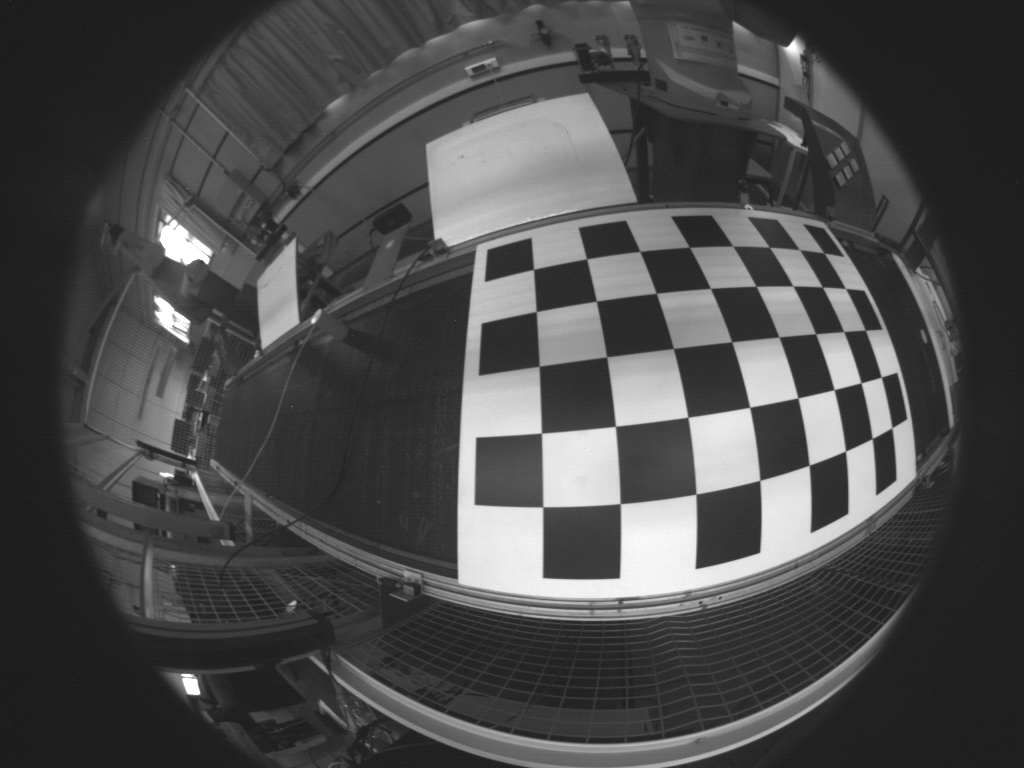
\includegraphics[width=.45\linewidth]{chessboard}
 \caption{Calibration landmarks, point grid with a low distortion camera (left) and OpenCV chessboard seen by a fish-eye camera (right).}
 \label{fig:landmarks}
\end{figure}

\newcommand{\xii}{{\boldsymbol{\xi}}}

In both cases, the interest points lie on a grid pattern of known dimension (rows, columns and inter-point distance). The 3D coordinates of those points
are thus known. The goal is to estimate the camera parameters $\xii$ and the camera poses $\M_i$ (one pose for each image) that minimize the reprojection error between the known 3D positions
and the extracted 2D (pixel) positions.

\subsection{Calibration procedure}
\label{sec:calib}

Calibration will begin by saving several images acquired from the camera (program \texttt{record}) The calibration program will then have to read them and extract the interest
points (already written in \texttt{calibration.cpp}). A virtual visual servoing scheme will then be used to minimize the error.
Assuming we are using $n$ images and that the calibration landmark is using $m$ points:
\begin{itemize}
 \item the reprojection error is of dimension $(2\times n\times m)$ (2 coordinates per point per image).
 \item the unknown is of dimension $(n_\xii + 6\times n)$ where $n_\xii$ is the number of parameters of the camera model.
\end{itemize}
The VVS is an optimization problem written as:
\begin{equation}\label{eq:calib}
 \xii, (\M_i)_i = \arg\min \norm{\s(\xii, (\M_i)_i) - \sd}^2
\end{equation}
where $\sd$ regroups the desired pixel coordinates of the interest points in each image and correspond to the extracted pixel positions, 
and where $\s(\xii, (\M_i)_i)$ is the pixel coordinates of the known 3D points when projected with intrinsic parameters $\xii$ and camera poses $(\M_i)_i$.

From an estimation of $\xii$ and $(\M_i)_i$, the 3D point $\X({}^o X,{}^o Y,{}^o Z)$ whom coordinates are expressed in the object frame $\Frame{o}$ can easily be projected in pixel coordinates.
The coordinates of $\X$ in the camera frame yield:
\begin{equation}\label{eq:framechange}
 \left[\begin{array}{c}{}^c\X\\1\end{array}\right]=   \left[\begin{array}{c}X\\Y\\Z\\1\end{array}\right] =\M_i\left[\begin{array}{c}\X\\1\end{array}\right]
\end{equation}

For a classical perspective camera model, we have $\xii = (p_x, p_y, u_0, v_0)$ and the perspective projection:
\begin{equation}\label{eq:projection}
 \left\{\begin{array}{ll}
  u &= p_x.X/Z + u_0 \\
  v &= p_y.Y/Z + v_0
 \end{array}\right.
\end{equation}

From \eqref{eq:framechange} and \eqref{eq:projection} the full projection function $\s(\xii, (\M_i)_i)$ can be defined.\\ 

\eqref{eq:calib} can then be resolved from an initial guess on $\xii$ and $(\M_i)_i$ with a simple gradient descent. 
The error derivative with regards to intrinsic parameters and camera poses has the following structure:
\newcommand{\der}{\text{d}}
\begin{equation}\label{eq:jacob}
 \der\s =  \left[\begin{array}{ccccc}
           \J_1 & \L_1 &  0 &  \hdots & 0 \\ 
           \J_i & 0 & \L_i &  \hdots & 0 \\
           \vdots& \vdots & \ddots & \ddots & \vdots\\
           \J_n & 0 & \hdots & 0 & \L_n
            \end{array}\right]
            \left[\begin{array}{c}\der\xii \\ \v_1 \\ \vdots \\ \v_n\end{array}\right]
             = \J\der\x
\end{equation}
where:
\begin{itemize}
\item $\J_i$ is the derivative of the reprojection of the points of image $i$ with regards to the intrinsic parameters (dimension $(2m)\times n_\xii$)
 \item $\L_i$ is the interaction matrix of the reprojection of the points of image $i$ (dimension $(2m)\times 6$)
 \item $\der\xii$ is the change in the intrinsic parameters (dimension $n_\xii$) 
 \item $\v_i$ is the velocity screw of the estimated camera pose of image $i$ (dimension $6$)
 \item As a consequence, $\J$ is of dimension $(2mn)\times (n_\xii+6n)$ and $\der\x$ is of dimension  $(n_\xii+6n)$
\end{itemize}
The gradient descent allows computing iteratively new values for $\xii$ and $(\M_i)_i$ with:
\begin{equation}
 \der\x = \left[\begin{array}{c}\der\xii \\ \v_1 \\ \vdots \\ \v_n\end{array}\right] = -\lambda\Jp(\s - \sd)
\end{equation}
The update of $\xii$ and $\M_i$ is then done with:
\begin{eqnarray}
 \xii^{\text{new}} =& \xii + \der\xii \label{upd:xi}\\
 \M_i^{\text{new}} =& \exp(-\v_i)\times\M_i \label{upd:M}
\end{eqnarray}
where $\exp(-\v_i)$ is the exponential map.\\

Matrices $\J_i$ and $\L_i$ are of course not constant and depend on the several considered points. The formulation of these matrices are given in Section \ref{sec:jacpersp} for a perspective camera.

\subsection{Pose computation procedure}
\label{sec:pose}
In pose computation we assume the camera is already calibrated and we are dealing with the image stream of the camera.
We are just looking for the current pose $\M$ of the camera.
The minimization problem is thus the same as \eqref{eq:calib} but is highly simplified:
\begin{equation}\label{eq:pose comp}
\M = \arg\min \norm{\s(\M) - \sd}^2
\end{equation}The exact same algorithm as for the calibration can thus be used, without having to consider intrinsic parameters or several images.
\eqref{eq:jacob} is simplified to :
\begin{equation}
 \der\s =  \L\v
\end{equation}
The initial guess for $\M$ still has to be done, but when a new image comes the guess is of course the previous estimation of $\M$ as we assume the image stream 
correspond to very close poses of the camera.

\subsection{Expected work}

During the lab the files will be modified and others will be created.
At the end of the lab, please send by email a zip file allowing to compile and test the program.

You may answer the questions by inserting comments in the code at the corresponding lines.
\newpage

\section{Calibration implementation}

You will first calibrate the camera you are working on. The first step is to save several images of the landmark (point grid) on the hard drive.

The files that need to be modified are:
\begin{itemize}
 \item \texttt{calibration.cpp}: main file, defines the image path, initial guess for the camera parameters and grid pattern (size, dimension)
 \item \texttt{perspective\_camera.h}: defines the camera model, you need to write how to project a point depending on the current camera parameters, and how to compute the Jacobian of these
 coordinates
 \item \texttt{vvs.cpp}: the \texttt{calibrate} method of this class has to be written according to the algorithm from Section \ref{sec:calib}.\\
 The overall architecture is already written, you have to write the content of the minimization loop:
 \begin{itemize}
  \item project a point from current estimation
  \item compute the Jacobians and write them into the global Jacobian
  \item  update the parameter estimation
 \end{itemize}
\end{itemize}

The calibration with virtual visual servoing is a highly non-linear, overconstrained algorithm. Indeed it tries to solve $2m\times n$ equations (2 coordinates for $m$ points in $n$ images) with
only $n_\xii + 6\times n$ unknown (the number of intrinsic parameters and 6 pose parameters for $n$ images). Hence, the initial guess is of great importance
not to fall in a local minimum. Here are some initial guess tips:
\begin{itemize}
 \item Camera parameters: we can assume a perspective camera with the middle pixel being on the optical axis, and a pixel dimension proportional to the image resolution. 
 A good initial guess could thus be written as:
 \begin{center}\cppstyle
\begin{lstlisting}
    // camera model with default parameters (in calibration.cpp)
    const double pxy = 0.5*(im[0].rows+im[0].cols);
    PerspectiveCamera cam(pxy, pxy, 0.5*im[0].cols, 0.5*im[0].rows);
\end{lstlisting}
\end{center}
\item Initial pose: as it uses Cartesian coordinates, the VVS is very sensible to big error on the rotation around Z. However as we know the points have been detected, the first row can be used to 
get a coarse estimation of this rotation. We also know that the object lies in front of the camera, which means a positive value for $t_z$. So a vector of $n$ homogeneous matrices could be initialized as:
 \begin{center}\cppstyle
\begin{lstlisting}
        M_.resize(n_im);
        // wild guess for initial pose, then will use the last found at initial value
        for(unsigned int n=0;n<n_im;++n)
            M_[n].buildFrom(0,0.,0.5,
            0,0,atan2(_cog[n][5].y-_cog[n][0].y, _cog[n][5].x-_cog[n][0].x));
\end{lstlisting}
\end{center}where we assume the camera is at 0.5 m from the object.
\end{itemize}

The calibration can be first carried with the point grid pattern, using the \texttt{GridTracker} class. You can then check that it also works on the chessboard, 
using the \texttt{CBTracker}. The detail of input/output for all classes and methods are found in Appendix \ref{sec:classes}.


\section{Pose computation implementation}

The source file for the pose computation does not exist, so you can copy and modify the \texttt{calibration.cpp} to a new file \texttt{posecomputation.cpp}\footnote{do not forget adding your new file 
to the CMakeLists.txt}. This time we do not want to load images from the hard drive but directly read them from the camera. This is possible with an infinite while loop and by using the \texttt{cv::VideoCapture} class.

For the pose computation, you can already initialize the camera with the parameters that have been found in the calibration. The files that need to be modified are then:
\begin{itemize}
 \item \texttt{posecomputation.cpp}: main file (has to be created), reads images from the camera, defines the grid pattern (size, dimension) and call the pose computation from VVS
 \item \texttt{perspective\_camera.h}: defines the camera model, it should be already done for the calibration 
 \item \texttt{vvs.cpp}: the \texttt{computePose} method of this class has to be written according to the algorithm from Section \ref{sec:pose}.
\end{itemize}
This time the initial guess is the same as above for the first image, but can be the previously found homogeneous matrix as the camera will not move too much between two images. This will allow the pose computation
converge faster.

\appendix

\section{Main classes}\label{sec:classes}

\subsection{OpenCV classes}

These labs use a few OpenCV classes, mainly images and points. The only one that needs to be used is the \texttt{cv::Point}, and basically we just have to know that the $(u,v)$ coordinates can be accessed
as \texttt{P.x} and \texttt{P.y}.

\subsection{ViSP classes}

This library includes many tools for linear algebra, especially for 3D transformations. These classes are mainly used inside the \texttt{VVS} class for the minimization algorithm.
The documentation is found here: \url{http://visp-doc.inria.fr/doxygen/visp-daily/classes.html}.\\
The main classes from ViSP (at least in this lab) are:
\begin{itemize}
\item \texttt{vpMatrix} represents a classical matrix, can then be transposed, inversed (or pseudo-inversed), multiplied with a vector, etc.
\item \texttt{vpColVector} is a column vector with classical mathematical properties.
\item \texttt{vpHomogeneousMatrix} represents a frame transformation matrix \texttt{M} and is initialized from 3 translation and 3 rotation parameters.
\item \texttt{vpPoint}: represents a 3D point in the world frame. If the world-to-camera pose is \texttt{M}, we can compute the point projection on the camera plane by:
\begin{center}\cppstyle
\begin{lstlisting}
        vpPoint P;
        vpHomogeneousMatrix M;
        P.track(M);
        double x = P.get_x();
        double y = P.get_y();
\end{lstlisting}
\end{center}
\end{itemize}


\subsection{Trackers}

The \texttt{CBTracker} and \texttt{GridTracker} are very similar and differ only from the object they try to detect. They have only two methods:
\begin{itemize}
    \item \texttt{bool detect(cv::Mat \&\_im, vector<cv::Point> \&\_cog)} \\ writes the vector of points \texttt{\_cog} with the points detected in image \texttt{\_im}
    \item \texttt{bool track(cv::Mat \&\_im, vector<cv::Point> \&\_cog)} \\ updates the vector of points \texttt{\_cog} with the points detected in image \texttt{\_im}.\\The update tries to 
    be consistent with the current values of the points, ie it will not lead to a 180${}^o$ rotation around Z.
\end{itemize}Both functions returns True if they managed to detect or track the points.
As for all visual trackers, we detect in the first image and track in the next images (except during calibration where there is no reason to track).\\
The tracker may be lost if the pattern is not here or if the image is blurry, so it can be a good idea to check the return value and re-detect points instead of always tracking them.

\subsection{Camera models}

The \texttt{GenericCamera} is a virtual class that implements the methods of any camera model:
\begin{itemize}
 \item \texttt{unsigned int nbParam()} \\ returns the number of parameters used by this camera model
 \item \texttt{void project(const vpPoint \&\_P, double \&\_u, double \&\_v)} \\ takes as an input the 3D point \texttt{\_P} that is already expressed in the camera frame, and computes the corresponding
 pixel coordinates $(u,v)$.
    \item \texttt{void computeJacobianIntrinsic(const vpPoint \&\_P, vpMatrix \&\_J)} \\ takes as an input the 3D point \texttt{\_P} that is already expressed in the camera frame and updates \texttt{\_J} so that it corresponds to the intrinsic Jacobian to be used in \eqref{eq:jacob}
    \item \texttt{void computeJacobianExtrinsic(const vpPoint \&\_P, vpMatrix \&\_L)} \\ takes as an input the 3D point \texttt{\_P} that is already expressed in the camera frame and updates \texttt{\_L} so that it corresponds to the extrinsic Jacobian to be used in \eqref{eq:jacob}
    \item \texttt{void updateIntrinsic(const vpColVector \&\_dxi)} \\ takes as input a small change of the intrinsic parameters and updates them according to \eqref{upd:xi}.
 \end{itemize}
 

 Two camera models are considered:
 
 \begin{enumerate}
  \item  \texttt{PerspectiveCamera}: Classical perspective camera, with projection equation \eqref{eq:projection}. The class is created but you will have to define the above mentionned methods (project, update Jacobian).
  \item \texttt{DistortionCamera}: Unified camera model, this class is already entirely written, you may use it to see how to define the methods for the perspective camera (of course the equations will be much more simple).
 \end{enumerate}
 
 \subsection{The \texttt{Pattern} structure}
 
 This structure is used to regroup data of a given image: the actual OpenCV image, the corresponding vector of points that have been extracted, and the window name used to display this image.
 
  \begin{center}\cppstyle
\begin{lstlisting}
 // structure used to regroup data
struct Pattern
{
    cv::Mat im;                     // OpenCV image
    std::vector<cv::Point> point;   // extracted points
    std::string window;             // window to display this image
};\end{lstlisting}
\end{center}This structure is only used to pass arguments to the virtual visual servoing class.


 \subsection{Virtual Visual Servoing class}
 
 The \texttt{VVS} class implements the minimization algorithm. It is instanciated with:
 \begin{center}\cppstyle
\begin{lstlisting}
        VVS vvs(cam, d, r, c);
\end{lstlisting}
\end{center}where cam is the camera model that is used (PerspectiveCamera or DistortionCamera) is the inter-point distances of the real landmark, and r and c are the number of rows and columns. The VVS uses these values to initialize the true position of the 3D points.

Only two methods are to be modified:
\begin{itemize}
    \item \texttt{void calibrate(std::vector<Pattern> \&\_pat)} (already quite written)\\ solves the calibration problem from a given set of \texttt{Pattern}. 
    \item \texttt{void computePose(Pattern \&\_pat, vpHomogeneousMatrix \&\_M, const bool \&\_reset)} \\ 
    solves the pose computation problem from a single \texttt{Pattern} (one image with extracted points).\\ This method can be highly inspired from the calibrate method, as shown in Section \ref{sec:pose}.
\end{itemize}

This class also have useful attributes:
\begin{itemize}
 \item \texttt{std::vector<vpPoint> X\_}: a vector of the true 3D position of the points, and is to be used in the reprojection error
 \item \texttt{GenericCamera* cam\_}: the camera that we are using or calibrating, it is a pointer to the methods can be called by using an arrow
\end{itemize}
As a syntax example, here is how we compute the (u,v) pixel coordinates of point k assuming a transformation matrix M (which can be quite useful for reprojection error):
 \begin{center}\cppstyle
\begin{lstlisting}
double u,v;
X_[k].track(M);		     // X_[k] is computed in the camera frame
cam_->project(X_[k], u, v);  // u and v are now the pixel coord. for the current camera model
\end{lstlisting}
\end{center}


\section{Jacobians for a perspective camera model}
\label{sec:jacpersp}

In this section we recall the intrinsic and extrinsic Jacobians for a classical camera model, with parameters $\xii = (p_x, p_y, u_0, v_0)$.
The projection model is:
\begin{equation}
 \left[\begin{array}{c}{}^c\X\\1\end{array}\right]=   \left[\begin{array}{c}X\\Y\\Z\\1\end{array}\right] =\M_i\left[\begin{array}{c}\X\\1\end{array}\right]
\end{equation}
\begin{equation}
 \left\{\begin{array}{ll}
  u &= p_x.X/Z + u_0  = p_x.x + u_0\\
  v &= p_y.Y/Z + v_0 = p_v.y + v_0
 \end{array}\right.
\end{equation}

The Jacobian of $(u,v)$ with regards to the intrinsic parameters is quite easy to compute:
\begin{equation}
 \J = \left[\begin{array}{cccc}
	    x & 0 & 1 & 0\\ 
	    0 & y & 0 & 1
            \end{array}\right]
\end{equation}
The Jacobian with regards to the extrinsic parameters (also called the interaction matrix) yields:
\begin{equation}
 \L =    \left[\begin{array}{cccccc}
-p_x/Z & 0 & p_x.x/Z & p_x.xy & -p_x(1+x^2) & p_x.y \\
0 & -p_y/Z & p_y.y/Z & p_y(1+y^2) & -p_y.xy & -p_y.x
\end{array}\right]            
\end{equation}
These two matrices should be defined in the \texttt{PerspectiveCamera::computeJacobianIntrinsic} and \texttt{PerspectiveCamera::computeJacobianExtrinsic}
methods, and depend of course on the considered point.




\end{document}
